%% EC5.407 Wireless Communications - Assignment 2 report
%% Build from this folder:  pdflatex report.tex && pdflatex report.tex
%% Figures and the tables of Appendix A are read from ../results, so the report
%% always shows the output of the submitted code.
\documentclass[11pt,a4paper]{article}

%% ---------------------------------------------------------------- packages
\usepackage[margin=2.2cm]{geometry}
\usepackage[T1]{fontenc}
\usepackage{lmodern}
\usepackage{microtype}
\usepackage{amsmath,amssymb}
\usepackage{graphicx}
\usepackage{booktabs,array}
\usepackage[font=small,labelfont=bf,labelsep=colon]{caption}
\usepackage[section]{placeins}          % keep floats inside their section
\usepackage{enumitem}
\usepackage{pgfplotstable}              % Appendix A tables straight from the CSV files
\usepackage[hidelinks]{hyperref}

\pgfplotsset{compat=1.18}
\graphicspath{{../results/}}
\setlength{\parindent}{0pt}
\setlength{\parskip}{5pt}
\setlist{itemsep=2pt,topsep=2pt,parsep=0pt}

%% ---------------------------------------------------------------- student details
\newcommand{\studentname}{Ande Karthik}
\newcommand{\rollnumber}{2023102009}

%% ---------------------------------------------------------------- notation
\newcommand{\snr}{\mathrm{SNR}}
\newcommand{\snrdb}{\mathrm{SNR}_{\mathrm{dB}}}
\newcommand{\CN}{\mathcal{CN}}
\newcommand{\E}{\mathbb{E}}
\newcommand{\norm}[1]{\lVert #1 \rVert}
\newcommand{\abs}[1]{\lvert #1 \rvert}
\newcommand{\Pe}{P_{\mathrm{e}}}
\newcommand{\hPe}{\hat{P}_{\mathrm{e}}}
\newcommand{\nerr}{n_{\mathrm{err}}}
\newcommand{\h}{\mathbf{h}}
\newcommand{\y}{\mathbf{y}}
\newcommand{\w}{\mathbf{w}}
\newcommand{\code}[1]{\texttt{\detokenize{#1}}}
\newcommand{\dB}{\,\mathrm{dB}}

%% ---------------------------------------------------------------- Appendix A tables
%% A simulated SER cell with fewer than 10 errors (written "k e-06" or "0" in the
%% CSV, since N = 10^6) shows the raw error count, e.g. "6 err."; these points are
%% not plotted. All other cells are printed in scientific notation.
\makeatletter
\def\ser@digit#1e-06#2\@nil{#1}
\def\ser@zero{0}
\newcommand{\simcell}[1]{%
  \def\ser@arg{#1}%
  \ifx\ser@arg\ser@zero
    \def\ser@cell{\textit{0 err.}}%
  \else
    \in@{e-06}{#1}%
    \ifin@
      \edef\ser@cell{\noexpand\textit{\ser@digit#1\@nil\space err.}}%
    \else
      \pgfmathprintnumberto[sci,sci zerofill,precision=2]{#1}{\ser@num}%
      \toks0=\expandafter{\ser@num}%
      \edef\ser@cell{\noexpand\ensuremath{\the\toks0}}%
    \fi
  \fi
  \pgfkeyslet{/pgfplots/table/@cell content}{\ser@cell}}
\makeatother
\pgfplotstableset{
  ser table/.style={
    col sep=comma,
    every last row/.style={after row=\bottomrule},
    display columns/0/.style={column name={$\snrdb$}, int detect, column type=c},
  },
  sim/.style={column name={sim.}, column type=r, assign cell content/.code={\simcell{##1}}},
  theory/.style={column name={theory}, column type=r, sci, sci zerofill, precision=2},
}

\begin{document}

%% ================================================================ title
\begin{center}
  {\LARGE EC5.407 Wireless Communications - Assignment 2}\\[5pt]
  {\large Detection and Diversity in AWGN and Fading Channels}\\[12pt]
  {\large \studentname \qquad \rollnumber}
\end{center}
\vspace{2pt}

%% ================================================================ set-up
\section{Simulation set-up (common to all problems)}
\label{sec:setup}

\subsection{Model and conventions}

All three problems use the conventions of the ``Getting Started'' section of the
assignment. The constellation has unit average energy, so the SNR is set only by
the noise variance:
\begin{equation*}
  E_s = \E\abs{x}^2 = \frac{1}{M}\sum_{i=1}^{M}\abs{u_i}^2 = 1, \qquad
  \E\abs{w}^2 = \frac{1}{\snr}, \qquad
  \snr = \frac{E_s}{\E\abs{w}^2}, \qquad \snr = 10^{\snrdb/10}.
\end{equation*}
\begin{itemize}
  \item \textbf{Constellations:} BPSK $\{+1, -1\}$ and 4-QAM
        $\{\pm A \pm jA\}$ with $A = 1/\sqrt2$. Both have unit energy, so they are
        compared at equal symbol energy.
  \item \textbf{Noise:} $w = \frac{1}{\sqrt{2\snr}}(w_I + jw_Q) \sim \CN(0, 1/\snr)$,
        with $w_I, w_Q \sim \mathcal{N}(0,1)$ independent.
  \item \textbf{Rayleigh fading:} $h = \frac{1}{\sqrt2}(h_I + jh_Q) \sim \CN(0,1)$, a new
        value for every symbol (for every Alamouti block in Problem~3), known at the
        receiver.
  \item \textbf{Monte Carlo size:} $N = 10^6$ symbols per SNR point, for every curve
        and every $L$.
  \item \textbf{Seed:} set once at the start of every script with
        \code{np.random.default_rng(2026)}.
  \item \textbf{Vectorised:} all $N$ symbols of an SNR point are processed at once. The
        only loops run over SNR points, schemes and $L$.
\end{itemize}

\subsection{Code structure}

Every block of the link in Fig.~1 of the assignment is written once, in \code{common/},
and every problem imports it. The code is Python~3.12 with NumPy, SciPy (only
\code{erfc}) and Matplotlib. No library function for modulation, detection or
error-rate calculation is used.

\begin{center}\small
  \begin{tabular}{@{}>{\raggedright\ttfamily}p{3.2cm}>{\raggedright\arraybackslash}p{12.8cm}@{}}
    \toprule
    \normalfont File & What it does \\
    \midrule
    constellation.py & BPSK and 4-QAM, normalised to $E_s = 1$. \\
    channel.py       & Complex Gaussian samples; AWGN, Rayleigh, $1 \times L$ SIMO and $2 \times 1$ MISO channels. \\
    detector.py      & One ML (minimum-distance) detector for any constellation,
                       $\hat\imath = \arg\min_m \abs{r - g\,u_m}^2$, computed for all $N$
                       samples at once as an $N \times M$ distance array. \\
    combining.py     & Receive combiners (none, MRC, SC) that turn the received samples
                       into one scalar decision statistic. \\
    simulation.py    & Algorithm~1: draw indices, send through the channel, combine,
                       detect, and count errors by comparing indices,
                       $\nerr = \sum_n \mathbf{1}\{\hat\imath_n \neq i_n\}$. \\
    theory.py        & $Q(a) = \tfrac12\,\mathrm{erfc}(a/\sqrt2)$ as its own function, the
                       formulas of the assignment table, and the exact 4-QAM SER of every
                       scheme (Sec.~\ref{sec:exact}). \\
    plotting.py\newline analysis.py & Figures (only points with $\nerr \ge 10$), CSV tables, SNR
                       gaps, slopes and $z$-scores. \\
    \midrule
    problem1/ to\newline problem3/ & One script per task. Each writes its figures, CSV table and
                       a \code{summary.txt} with every number quoted below to
                       \code{results/q1} -- \code{results/q3}. \\
    overall\_check.py & Compares every plotted point of all problems with its exact
                       theory (Sec.~\ref{sec:check}). \\
    \bottomrule
  \end{tabular}
\end{center}

\textbf{One detector for every receiver.} Every receiver in this assignment reduces
what it receives to an equivalent scalar channel
\begin{equation}
  r = g\,x + n, \qquad n \sim \CN(0, 1/\snr), \qquad g \text{ known at the receiver}.
  \label{eq:scalar}
\end{equation}
The ML detector of Problem~1 is then applied without change; only the gain $g$
differs: $g = 1$ (AWGN), $g = h$ (fading), $g = \norm{\h}$ (MRC and beamforming),
$g = h_{\ell^\star}$ (SC) and $g = \norm{\h}/\sqrt2$ (Alamouti). The MRC and
Alamouti outputs are divided by $\norm{\h}$ so that the noise variance is $1/\snr$
in every case. Without this division the gains would be $\norm{\h}^2$ and
$\norm{\h}^2/\sqrt2$, with noise variance $\norm{\h}^2/\snr$. The SNR and the
decisions would be the same (Sec.~\ref{sec:p2-statistics}).

\textbf{Reproducing.} Each script is run as a module from the code root, for
example \code{python3 -m problem2.receive_diversity}; the README lists all
commands. Each script takes under a minute and reproduces its figures and numbers
exactly.

\subsection{How accurate is a simulated point?}
\label{sec:accuracy}

A simulated point is $\hPe = \nerr/N$. Each symbol is an independent
Bernoulli($\Pe$) trial, so $\mathrm{std}(\hPe) = \sqrt{\Pe(1-\Pe)/N}$, and the
relative accuracy is about $1/\sqrt{\nerr}$:
\begin{center}\small
  \begin{tabular}{@{}lcccc@{}}
    \toprule
    errors observed, $\nerr$ & 10 & 100 & 1000 & 10\,000 \\
    relative accuracy        & $\pm32\%$ & $\pm10\%$ & $\pm3\%$ & $\pm1\%$ \\
    \bottomrule
  \end{tabular}
\end{center}
A difference between simulation and theory is measured in units of this
standard deviation,
\begin{equation}
  z = \frac{\hPe - \Pe}{\sqrt{\Pe(1-\Pe)/N}}.
  \label{eq:z}
\end{equation}
If the simulation is correct, $z$ behaves like a standard normal variable. Most
points then have $\abs{z} < 2$, and the worst of a few hundred points is close
to 3.

\subsection{Exact 4-QAM theory used for checking}
\label{sec:exact}

The assignment table gives an exact formula for BPSK in fading but only an
approximation for 4-QAM, and no formula for Problems~2 and~3. To check every
curve against an exact value, I compute the exact 4-QAM SER of each scheme in
three steps.
\begin{enumerate}
  \item \textbf{Every scheme is an AWGN channel with a random gain.} By
        \eqref{eq:scalar}, the SNR after detection is $\gamma\,\snr$ with
        $\gamma = \abs{g}^2$ (table below).
  \item \textbf{Error probability for a fixed gain.} 4-QAM is two independent BPSK
        decisions (I and Q), each with half the energy:
        $\Pe(\gamma) = 2Q\big(\sqrt{\gamma\snr}\big) - Q^2\big(\sqrt{\gamma\snr}\big)$.
  \item \textbf{Average over the gain.} Craig's forms of the $Q$-function,
        \begin{equation*}
          Q(x) = \frac1\pi\int_0^{\pi/2} e^{-x^2/(2\sin^2\theta)}\,d\theta, \qquad
          Q^2(x) = \frac1\pi\int_0^{\pi/4} e^{-x^2/(2\sin^2\theta)}\,d\theta,
        \end{equation*}
        turn the average into one that only needs the moment-generating function
        $M_\gamma(s) = \E[e^{-s\gamma}]$:
        \begin{equation}
          \Pe = \frac{2}{\pi}\int_0^{\pi/2} M_\gamma\Big(\frac{\snr}{2\sin^2\theta}\Big)d\theta
              - \frac{1}{\pi}\int_0^{\pi/4} M_\gamma\Big(\frac{\snr}{2\sin^2\theta}\Big)d\theta .
          \label{eq:craig}
        \end{equation}
\end{enumerate}

\begin{center}\small
  \begin{tabular}{@{}llll@{}}
    \toprule
    Scheme & Gain $\gamma = \abs{g}^2$ & Distribution & $M_\gamma(s)$ \\
    \midrule
    Single antenna        & $\abs{h}^2$                   & $\mathrm{Exp}(1)$     & $1/(1+s)$ \\
    MRC ($L$), beamforming ($L=2$) & $\norm{\h}^2$        & $\mathrm{Gamma}(L,1)$ & $(1+s)^{-L}$ \\
    SC ($L$)              & $\max_\ell\abs{h_\ell}^2$     & same as $\sum_{k=1}^{L} E_k/k$, $E_k \sim \mathrm{Exp}(1)$ & $\prod_{k=1}^{L} k/(k+s)$ \\
    Alamouti              & $\norm{\h}^2/2$               & $\tfrac12\,\mathrm{Gamma}(2,1)$ & $(1+s/2)^{-2}$ \\
    \bottomrule
  \end{tabular}
\end{center}

The integrals in \eqref{eq:craig} are evaluated with 256-point Gauss--Legendre
quadrature (\code{ser_qam4_fading_mgf} in \code{theory.py}). I checked them in two
ways:
\begin{itemize}
  \item For one antenna, the result equals the closed form derived the same way,
        $\Pe = (1-\mu) - \tfrac14\big[1 - \tfrac4\pi\,\mu\arctan(1/\mu)\big]$ with
        $\mu = \sqrt{(\snr/2)/(1+\snr/2)}$.
  \item For MRC and SC with $L = 2, 4$, the result agrees with direct numerical
        integration over the density of $\gamma$ to machine precision.
\end{itemize}

\subsection{Overall check of all simulations}
\label{sec:check}

The script \code{overall_check.py} compares every plotted point ($\nerr \ge 10$) of
Problems~1--3 with its exact value $p$, using the $z$-score \eqref{eq:z}, written
with error counts as
\begin{equation*}
  z = \frac{\nerr - Np}{\sqrt{Np(1-p)}} .
\end{equation*}
If the simulation is unbiased, $z$ behaves like a standard normal variable.

Three curves use exactly the same random numbers: MRC and SC with $L = 1$
(Problem~2), and the single-antenna curve of Problem~3. Both scripts start from
seed 2026 and draw the symbols, channels and noise in the same order. Their error
counts are identical, so they are counted \emph{once}. This leaves 160 independent
points (Table~\ref{tab:check}).

\begin{table}[htbp]
  \centering\small
  \caption{Agreement between every simulated curve and its exact theory
           (\code{results/overall_check.txt}). ``Max $\abs{z}$'' is the largest
           deviation over the plotted points of the curve. $^\ast$\,This row also
           stands for SC, $L = 1$ and the single-antenna curve of Problem~3 (same
           random numbers, identical error counts).}
  \label{tab:check}
  \begin{tabular}{@{}llcc@{\hspace{1.0cm}}llcc@{}}
    \toprule
    Problem & Curve & Points & Max $\abs{z}$ & Problem & Curve & Points & Max $\abs{z}$ \\
    \midrule
    1 & BPSK, AWGN       & 10 & 2.59 & 2 & MRC, $L = 4$    &  8 & 2.01 \\
    1 & 4-QAM, AWGN      & 13 & 1.95 & 2 & SC, $L = 2$     & 13 & 1.64 \\
    1 & BPSK, fading     & 21 & 3.02 & 2 & SC, $L = 4$     &  9 & 1.12 \\
    1 & 4-QAM, fading    & 21 & 1.78 & 3 & Beamforming     & 13 & 2.06 \\
    2 & MRC, $L = 1$\,$^\ast$ & 13 & 1.85 & 3 & Alamouti   & 13 & 2.55 \\
    2 & MRC, $L = 2$     & 13 & 1.03 & 3 & MRC, $L = 2$    & 13 & 1.85 \\
    \bottomrule
  \end{tabular}
\end{table}

Table~\ref{tab:check-stats} compares the statistics of all 160 $z$-values with
those of a standard normal variable.

\begin{table}[htbp]
  \centering\small
  \caption{Statistics of $z$ over all 160 independent plotted points.}
  \label{tab:check-stats}
  \begin{tabular}{@{}lcc@{}}
    \toprule
    Statistic over all 160 points & Measured & Expected if unbiased \\
    \midrule
    points with $\abs{z} < 1$ & 71.2\% & 68.3\% \\
    points with $\abs{z} < 2$ & 95.0\% & 95.4\% \\
    points with $\abs{z} < 3$ & 99.4\% & 99.7\% \\
    largest $\abs{z}$         & 3.02   & reached by chance in 33\% of runs \\
    mean of $z$ (bias)        & $+0.079$ & $0 \pm 0.08$ \\
    mean of $z^2$             & 0.97   & $1 \pm 0.11$ \\
    \bottomrule
  \end{tabular}
\end{table}

\textbf{Conclusion.} Every simulated curve agrees with its exact theory, and the
160 deviations are spread exactly like Monte Carlo noise should be. The share of
points within $1\sigma$, $2\sigma$ and $3\sigma$ matches the normal distribution,
the mean of $z$ shows no bias, and the mean of $z^2$ is 1 within its accuracy. The
largest deviation, $3.02\sigma$ (BPSK in fading at 6~dB, $+1.3\%$), is the only
point beyond $3\sigma$. For 160 independent points, a maximum this large happens
by chance in about one run in three. The only \emph{systematic} difference in
this report is between the 4-QAM fading simulation and the \emph{approximate}
formula of the assignment table, explained in Sec.~\ref{sec:p1-agreement}.

%% ================================================================ problem 1
\section{Problem 1 --- SER in AWGN and Rayleigh fading}
\label{sec:p1}

Problem~1 measures the SER of BPSK and 4-QAM over the channel
\begin{equation}
  y = hx + w, \qquad x \in \mathcal{X}, \qquad w \sim \CN(0, 1/\snr),
  \label{eq:p1-channel}
\end{equation}
with $h = 1$ in Task~1 (AWGN) and $h \sim \CN(0,1)$ in Task~2 (Rayleigh fading). Both
tasks use the unit-energy constellations, the ML detector and the error counting of
Sec.~\ref{sec:setup}. In both channels the receiver knows $h$, so the ML decision is
\begin{equation}
  \hat\imath = \arg\min_{i} \abs{y - h\,u_i}^2 .
  \label{eq:p1-ml}
\end{equation}
Each task below first derives the theoretical SER, then describes the simulation and
shows its figure. The results are discussed in Sec.~\ref{sec:p1-discussion}.

\subsection{Task 1: AWGN channel}
\label{sec:p1-task1}

\textbf{Theoretical expressions.} With $h = 1$ the receiver sees $y = x + w$. The
real and imaginary parts of $w$ are independent, each $\mathcal{N}\big(0, 1/(2\snr)\big)$.
The Gaussian tail function $Q(a) = \tfrac12\,\mathrm{erfc}(a/\sqrt2)$ is implemented as its
own function (\code{qfunc}).
\begin{itemize}
  \item \textbf{BPSK.} The points $\pm1$ are separated by the threshold
        $\mathrm{Re}\{y\} = 0$, at distance 1 from each point. An error happens when the
        real part of the noise is larger than 1 in the wrong direction:
        \begin{equation}
          \Pe^{\mathrm{BPSK}} = \Pr\Big[\mathcal{N}\big(0, \tfrac{1}{2\snr}\big) > 1\Big]
                            = Q\big(\sqrt{2\snr}\big).
          \label{eq:p1-awgn-bpsk}
        \end{equation}
  \item \textbf{4-QAM.} The points $(\pm1 \pm j)/\sqrt2$ are two BPSK signals, one on I and
        one on Q, each with amplitude $1/\sqrt2$ (half the energy) and its own
        independent noise. One component is wrong with probability
        $q = Q\big((1/\sqrt2)\big/\sqrt{1/(2\snr)}\big) = Q(\sqrt{\snr})$. The symbol is
        correct only if both components are correct:
        \begin{equation}
          \Pe^{\mathrm{4QAM}} = 1 - (1-q)^2 = 2Q\big(\sqrt{\snr}\big) - Q^2\big(\sqrt{\snr}\big).
          \label{eq:p1-awgn-qam}
        \end{equation}
        An error in one or in both components counts as one symbol error.
\end{itemize}

\textbf{Simulation.} The script \code{problem1/awgn_ser.py} runs Algorithm~1 for
$\snrdb \in \{0, 1, \dots, 12\}$. For each modulation and SNR it draws $N = 10^6$
equiprobable indices, sends $x = u_i$ through $y = x + w$, detects with
\eqref{eq:p1-ml} and counts the errors. The expressions \eqref{eq:p1-awgn-bpsk} and
\eqref{eq:p1-awgn-qam} are evaluated at the same SNR points. Fig.~\ref{fig:awgn}
shows both schemes on one figure: simulation as markers, theory as lines.

\begin{figure}[htbp]
  \centering
  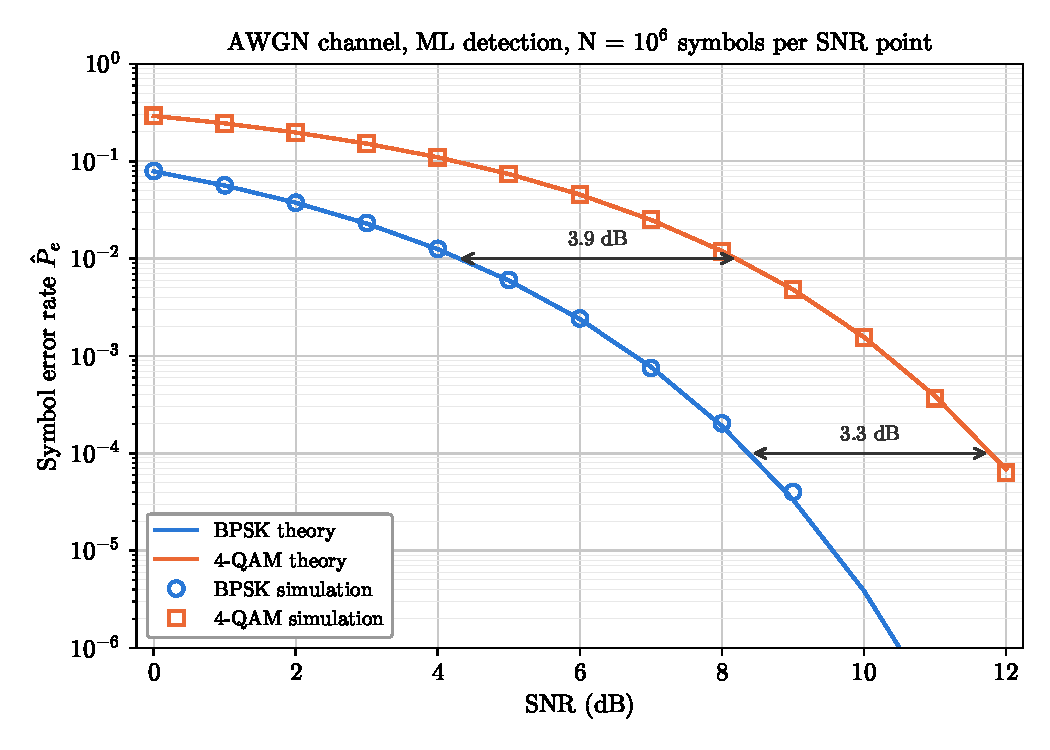
\includegraphics[width=0.74\linewidth]{q1/awgn_ser.pdf}
  \caption{Problem~1, Task~1: SER of BPSK and 4-QAM in the AWGN channel ($h = 1$)
           with ML detection. Markers: Monte Carlo simulation with $N = 10^6$
           symbols per SNR point, $\snrdb \in \{0, 1, \dots, 12\}$; only points with
           $\nerr \ge 10$ are shown. Lines: theory \eqref{eq:p1-awgn-bpsk} and
           \eqref{eq:p1-awgn-qam}. Arrows: the
           measured SNR gap between the two schemes, 3.9~dB at $10^{-2}$ and 3.3~dB at
           $10^{-4}$. \textbf{The BPSK--4-QAM gap is not constant: it shrinks towards
           3~dB as the SNR grows} (Sec.~\ref{sec:p1-gaps}).}
  \label{fig:awgn}
\end{figure}

\subsection{Task 2: Rayleigh fading channel}
\label{sec:p1-task2}

\textbf{Channel.} A new $h \sim \CN(0,1)$ is drawn for every symbol and is known at
the receiver (coherent detection). For a given $h$, the link is an AWGN link whose
SNR is multiplied by the channel power gain $g = \abs{h}^2$. Since $h \sim \CN(0,1)$,
$g$ is exponential, $f_g(g) = e^{-g}$ for $g \ge 0$, with $\E[g] = 1$. So $\snr$ is
also the average received SNR.

\textbf{Theoretical expressions.} Each fading result is the AWGN result for a fixed
$g$, averaged over the distribution of $g$.
\begin{itemize}
  \item \textbf{BPSK.} For a fixed $g$, \eqref{eq:p1-awgn-bpsk} becomes
        $Q\big(\sqrt{2g\snr}\big)$. Averaging over $g$ gives:
        \begin{equation}
          \Pe^{\mathrm{BPSK}} = \int_0^\infty Q\big(\sqrt{2g\snr}\big)\,e^{-g}\,dg
          = \frac12\Big(1 - \sqrt{\frac{\snr}{1+\snr}}\Big).
          \label{eq:p1-ray-bpsk}
        \end{equation}
  \item \textbf{4-QAM, formula of the assignment table.} Twice the BPSK result at half
        the SNR:
        \begin{equation}
          \Pe^{\mathrm{4QAM}} \approx 2\cdot\frac12\Big(1 - \sqrt{\frac{\snr/2}{1+\snr/2}}\Big).
          \label{eq:p1-ray-qam}
        \end{equation}
        This is the probability of an I error plus the probability of a Q error. It
        leaves out the event that both are wrong, so it is an approximation (an upper
        bound).
  \item \textbf{4-QAM, exact (extra, for checking).} Averaging the complete AWGN
        expression \eqref{eq:p1-awgn-qam}, with $q = Q\big(\sqrt{g\snr}\big)$, over $g$
        gives, with Craig's formula (Sec.~\ref{sec:exact}),
        \begin{equation}
          \Pe^{\mathrm{4QAM}} = \int_0^\infty \big[2q - q^2\big]\,e^{-g}\,dg
          = (1-\mu) - \tfrac14\Big[1 - \tfrac4\pi\,\mu\arctan\tfrac1\mu\Big],
          \qquad \mu = \sqrt{\frac{\snr/2}{1+\snr/2}} .
          \label{eq:p1-ray-exact}
        \end{equation}
        The first term, $1-\mu$, is exactly the table formula \eqref{eq:p1-ray-qam}; the
        second is the dropped ``both wrong'' term. This curve is only used to explain
        the simulated 4-QAM points; the comparison asked for in Task~2 uses
        \eqref{eq:p1-ray-qam}.
\end{itemize}

\textbf{Simulation.} The script \code{problem1/rayleigh_ser.py} runs Algorithm~1 for
$\snrdb \in \{0, 2, \dots, 40\}$, with a fresh $h$ and $w$ for every symbol and
$N = 10^6$ symbols per modulation and SNR point. The detector \eqref{eq:p1-ml} uses
the known $h$. Fig.~\ref{fig:rayleigh} shows the simulation with the expressions
\eqref{eq:p1-ray-bpsk}--\eqref{eq:p1-ray-exact}. Fig.~\ref{fig:awgn-vs-fading} is an
extra figure that places the AWGN theory of Task~1 next to the fading results; it is
used in the discussion of Sec.~\ref{sec:p1-deep-fade}.

\begin{figure}[htbp]
  \centering
  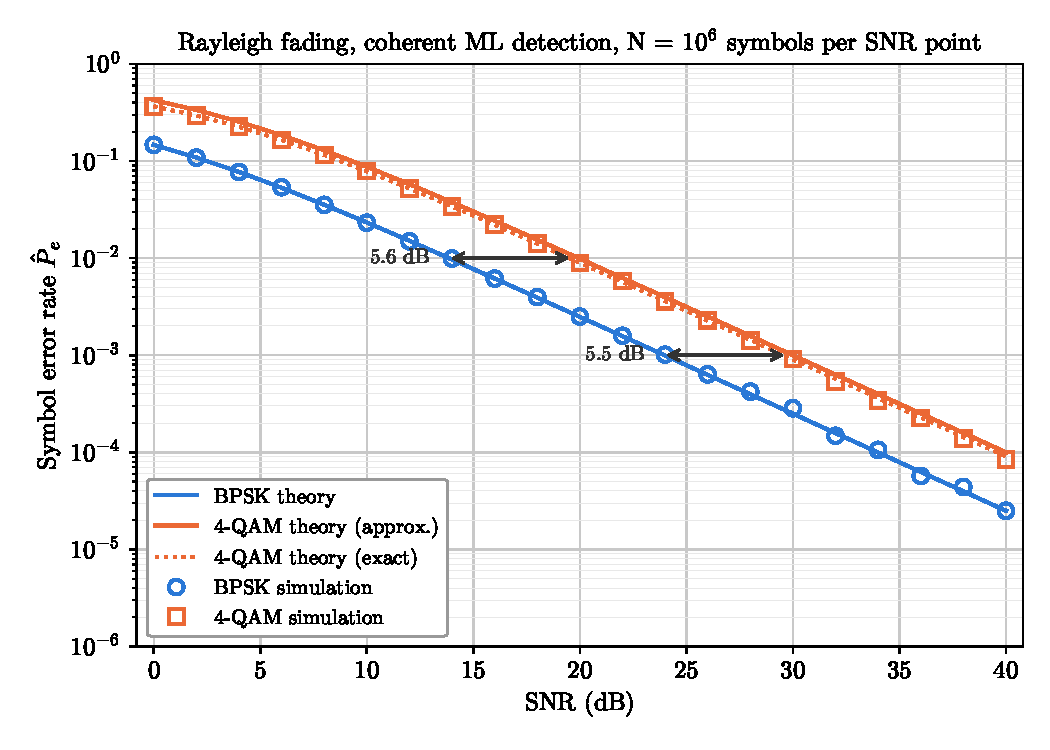
\includegraphics[width=0.74\linewidth]{q1/rayleigh_ser.pdf}
  \caption{Problem~1, Task~2: SER of BPSK and 4-QAM in Rayleigh fading with coherent
           ML detection. Markers: simulation with $N = 10^6$ symbols per SNR point,
           $\snrdb \in \{0, 2, \dots, 40\}$, points with $\nerr \ge 10$. Solid lines:
           assignment table \eqref{eq:p1-ray-bpsk} and \eqref{eq:p1-ray-qam} (an
           approximation for 4-QAM). Dotted: exact 4-QAM SER \eqref{eq:p1-ray-exact}.
           Arrows: the measured
           BPSK--4-QAM gap, 5.6~dB at $10^{-2}$ and 5.5~dB at $10^{-3}$.
           \textbf{The gap is nearly constant, about 5.5~dB: both curves are parallel
           lines of slope $\boldsymbol{-1}$} (Sec.~\ref{sec:p1-gaps}).}
  \label{fig:rayleigh}
\end{figure}

\begin{figure}[htbp]
  \centering
  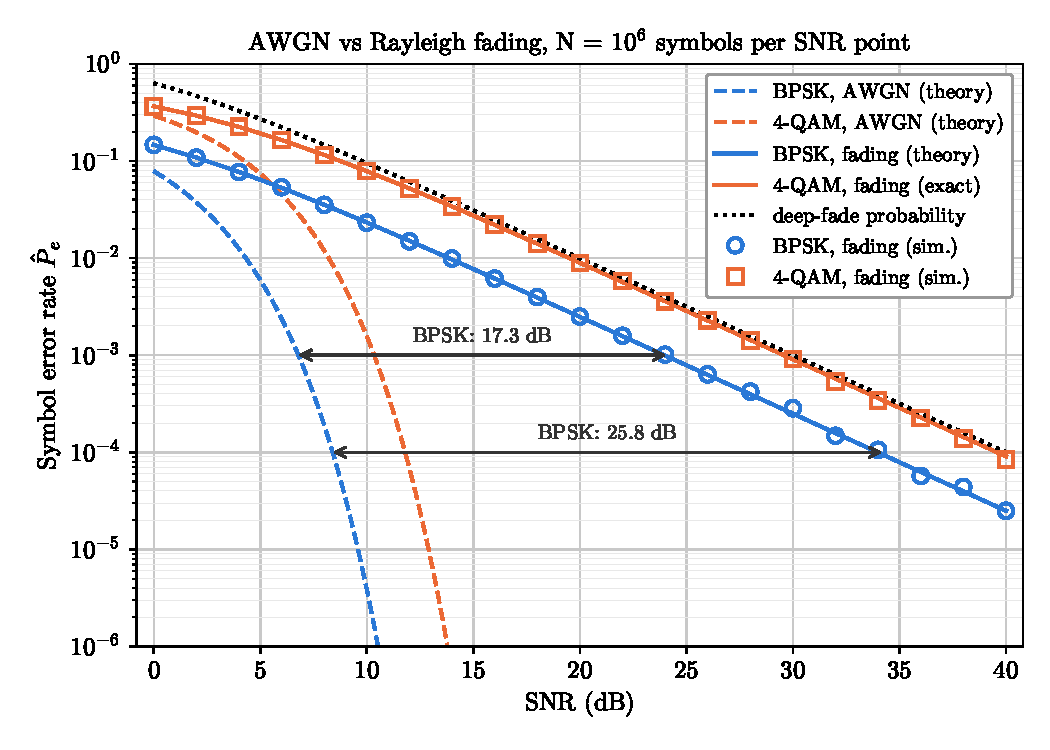
\includegraphics[width=0.74\linewidth]{q1/awgn_vs_rayleigh.pdf}
  \caption{Extra figure: AWGN (dashed, theory) against Rayleigh fading (solid lines:
           theory; markers: the simulation of Fig.~\ref{fig:rayleigh}, $N = 10^6$
           symbols per SNR point, 0--40~dB). Dotted: deep-fade probability
           $\Pr[\abs{h}^2\snr < 1] = 1 - e^{-1/\snr} \approx 1/\snr$. Arrows: the extra
           SNR that BPSK needs in fading, 17.3~dB at $10^{-3}$ and 25.8~dB at
           $10^{-4}$. \textbf{The AWGN--fading gap is not constant: it grows as the
           target SER falls} (Sec.~\ref{sec:p1-gaps}).}
  \label{fig:awgn-vs-fading}
\end{figure}

\FloatBarrier   % all three figures before the discussion
\subsection{Discussion}
\label{sec:p1-discussion}

The assignment asks for two points: the agreement between simulation and theory,
with the reason for any deviation (Sec.~\ref{sec:p1-agreement}), and the difference
between the AWGN and fading curves at high SNR, explained with the deep-fade argument
(Sec.~\ref{sec:p1-deep-fade}). Sec.~\ref{sec:p1-gaps} explains the gaps marked by the
arrows in Figs.~\ref{fig:awgn}--\ref{fig:awgn-vs-fading}.

\subsubsection{Agreement between simulation and theory}
\label{sec:p1-agreement}

\begin{itemize}
  \item \textbf{AWGN (Fig.~\ref{fig:awgn}, Table~\ref{tab:a-awgn}).} Both schemes
        match theory: max $\abs{z}$ is 2.59 (BPSK) and 1.95 (4-QAM). The largest
        \emph{relative} deviations occur where few errors are seen. For example, BPSK
        at 9~dB has 40 errors where 33.6 are expected ($+19\%$, only $1.1\sigma$).
        At 10, 11 and 12~dB, BPSK gives 6, 0 and 0 errors (3.9, 0.26 and 0.01
        expected). These points are not plotted (G.7): $10^6$ symbols cannot
        measure such small error rates.
  \item \textbf{Fading, BPSK.} The simulation follows the exact formula
        $\tfrac12\big(1 - \sqrt{\snr/(1+\snr)}\big)$, within $\pm2.5\%$ wherever
        $\nerr > 1000$. With fewer errors the scatter grows, as the table of
        Sec.~\ref{sec:accuracy} predicts. The largest relative deviation is $+14\%$ at 30~dB (284
        errors against 250 expected, $2.2\sigma$).
  \item \textbf{Fading, 4-QAM: a systematic deviation from the table formula.} The
        simulated SER is \emph{below} the table formula at every SNR: 13.5\% lower at
        0~dB and 7--11\% lower from 10 to 30~dB. That is up to $116\sigma$, so it is
        not noise. The simulation is not wrong: it matches the \emph{exact} curve
        (dotted in Fig.~\ref{fig:rayleigh}, max $\abs{z} = 1.78$). The reasons:
        \begin{itemize}
          \item Per symbol, the error probability is $2q - q^2$ with
                $q = Q(\sqrt{\abs{h}^2\snr})$ the error probability of one component.
                The table formula keeps only $\E[2q]$ and drops $-\E[q^2]$, the event
                that I \emph{and} Q are both wrong. It is therefore an upper bound.
          \item In AWGN, $q^2 \ll q$ at high SNR, so the dropped term does not matter.
                In fading it does: errors happen mostly in deep fades, and there both
                components see the same small $\abs{h}$ and fail together.
          \item At high SNR, $\E[2q] \to 1/\snr$ and
                $\E[q^2] \to \tfrac14\big(1 - \tfrac2\pi\big)/\snr = 0.091/\snr$. The
                exact SER is therefore $0.909/\snr$, and the table formula is 10\% too
                high. The simulation output confirms this: the formula exceeds the
                exact value by 15.8\% at 0~dB and by 10.0\% from 30~dB on.
          \item On the dB axis this is only $10\log_{10}(1/0.909) = 0.41$~dB, which is
                why the two lines look so close in Fig.~\ref{fig:rayleigh}.
        \end{itemize}
\end{itemize}

\subsubsection{AWGN versus fading at high SNR: the deep-fade argument}
\label{sec:p1-deep-fade}

\textbf{What the figures show.}
\begin{itemize}
  \item \emph{AWGN:} the SER falls \emph{exponentially} with SNR, because
        $Q(x) \le \tfrac12 e^{-x^2/2}$. The curves are a steep ``waterfall'': BPSK
        goes from $10^{-3}$ at 6.8~dB to $10^{-4}$ at 8.4~dB, one decade in only
        1.6~dB.
  \item \emph{Rayleigh fading:} the curves become straight lines of slope $-1$, so
        $\Pe \propto \snr^{-1}$: one decade per 10~dB. The fitted slope over
        30--40~dB is 1.02 for both schemes. At high SNR,
        $\Pe^{\mathrm{BPSK}} \approx 1/(4\snr)$ and $\Pe^{\mathrm{4QAM}} \approx 0.909/\snr$.
\end{itemize}

\textbf{Why: errors come from deep fades.}
\begin{enumerate}
  \item For a given channel, the link is an AWGN link whose SNR is scaled by
        $\abs{h}^2$: $\Pe(h) = Q\big(\sqrt{2\abs{h}^2\snr}\big)$ for BPSK.
  \item This gives two regimes:
        \begin{itemize}
          \item if $\abs{h}^2\snr \gg 1$, $\Pe(h)$ is exponentially small, so good
                channels contribute almost no errors;
          \item if $\abs{h}^2\snr \lesssim 1$ (a \emph{deep fade}), $\Pe(h)$ is of order
                one (at least $Q(\sqrt2) = 0.079$).
        \end{itemize}
  \item Because $\abs{h}^2 \sim \mathrm{Exp}(1)$, a deep fade is not rare:
        \begin{equation*}
          \Pr\big[\abs{h}^2 < 1/\snr\big] = 1 - e^{-1/\snr} \approx \frac{1}{\snr}.
        \end{equation*}
        This is the dotted line in Fig.~\ref{fig:awgn-vs-fading}. It runs right along
        the fading curves, with the same slope.
  \item Hence $\Pe \approx \Pr[\text{deep fade}] \times O(1) \propto 1/\snr$. More
        transmit power makes deep fades only proportionally rarer, so the SER also
        falls only linearly.
\end{enumerate}

\textbf{Simulation evidence.} The Problem~1 script also records $\abs{h}^2\snr$ for
every BPSK symbol and checks which errors happen during a deep fade
(\code{results/q1/rayleigh_summary.txt}):
\begin{center}\small
  \begin{tabular}{@{}lcccc@{}}
    \toprule
    $\snrdb$ & 10 & 20 & 30 & 40 \\
    \midrule
    symbols sent in a deep fade         & 9.5\% & 1.0\% & 0.10\% & 0.010\% \\
    errors (out of $10^6$ symbols)      & 23\,570 & 2\,506 & 236 & 24 \\
    errors that happened in a deep fade & 77\% & 74\% & 70\% & 83\% \\
    \bottomrule
  \end{tabular}
\end{center}
Only about $1/\snr$ of the symbols are sent in a deep fade, yet these few
symbols cause about three quarters of all errors at every SNR.

\textbf{The price of fading.} SNR needed for a target SER:
\begin{center}\small
  \begin{tabular}{@{}llccc@{}}
    \toprule
    Scheme & Target $\Pe$ & AWGN (theory) & Rayleigh (simulation) & Extra SNR needed \\
    \midrule
    BPSK  & $10^{-3}$ & 6.8~dB  & 24.1~dB & 17.3~dB \\
    BPSK  & $10^{-4}$ & 8.4~dB  & 34.2~dB & 25.8~dB \\
    4-QAM & $10^{-3}$ & 10.4~dB & 29.6~dB & 19.2~dB \\
    4-QAM & $10^{-4}$ & 11.8~dB & 39.3~dB & 27.5~dB \\
    \bottomrule
  \end{tabular}
\end{center}
The penalty grows as the target SER falls (arrows in Fig.~\ref{fig:awgn-vs-fading}).
Reducing it is the purpose of the diversity schemes of Problems~2 and~3.

\subsubsection{Gaps between the curves (arrows in the figures)}
\label{sec:p1-gaps}

\begin{itemize}
  \item \textbf{BPSK versus 4-QAM in AWGN: not constant} (Fig.~\ref{fig:awgn}).
        Measured: 3.87~dB at $10^{-2}$, 3.54~dB at $10^{-3}$ and 3.30~dB at
        $10^{-4}$ (theory 3.89, 3.56 and 3.40~dB).
        \begin{itemize}
          \item At equal symbol energy, each 4-QAM component has half the energy of a
                BPSK symbol: $Q(\sqrt{\snr})$ against $Q(\sqrt{2\snr})$. That alone is
                a shift of exactly 3~dB.
          \item 4-QAM also has the factor 2 in front of $Q(\cdot)$ (either component can
                fail). On a steep waterfall this factor costs only a small extra SNR,
                which shrinks as the SNR grows, so the gap tends to 3.01~dB.
        \end{itemize}
  \item \textbf{BPSK versus 4-QAM in fading: constant, about 5.6~dB}
        (Fig.~\ref{fig:rayleigh}). Measured: 5.56~dB at $10^{-2}$ and 5.53~dB at
        $10^{-3}$ (exact theory 5.66 and 5.61~dB). At $10^{-4}$ the measured value,
        5.11~dB, is less accurate: there the 4-QAM curve is read between its last two
        points, with only 138 and 84 errors.
        \begin{itemize}
          \item Both curves have slope $-1$, so at high SNR they are parallel,
                $\Pe \approx c/\snr$, and only the constant $c$ depends on the
                modulation: $c = 0.25$ for BPSK and $0.909$ for 4-QAM. The offset is
                $10\log_{10}(0.909/0.25) = 5.61$~dB.
          \item The offset is larger than in AWGN because on a slope-$1$ line a factor
                in front of the SER is never small. Half the energy per component
                doubles $c$ (3.01~dB), two components double it again (3.01~dB), and
                the joint-error term removes 9\% ($-0.41$~dB).
        \end{itemize}
  \item \textbf{AWGN versus fading: not constant, it grows}
        (Fig.~\ref{fig:awgn-vs-fading}). For BPSK it is 17.3~dB at $10^{-3}$ and
        25.8~dB at $10^{-4}$. One curve falls exponentially and the other as
        $1/\snr$, so they cannot be parallel.
\end{itemize}

%% ================================================================ problem 2
\section{Problem 2 --- Receive diversity (SIMO \texorpdfstring{$1 \times L$}{1 x L}), 4-QAM}
\label{sec:p2}

Problem~2 adds $L$ receive antennas to the fading channel of Problem~1. One transmit
antenna sends a 4-QAM symbol $x$, and the receiver collects
\begin{equation}
  \y = \h x + \w, \qquad
  \h = (h_1, \dots, h_L)^\top, \qquad
  \w = (w_1, \dots, w_L)^\top .
  \label{eq:p2-channel}
\end{equation}
\begin{itemize}
  \item \textbf{Channel:} $h_\ell \sim \CN(0,1)$, independent across antennas and drawn
        again for every symbol. The receiver knows $\h$.
  \item \textbf{Noise:} $w_\ell \sim \CN(0, 1/\snr)$, independent across antennas and
        independent of $\h$.
  \item \textbf{SNR:} since $\E\abs{h_\ell}^2 = \E\abs{x}^2 = 1$, $\snr$ is the average
        SNR \emph{per receive antenna}. For $L = 1$ the model is exactly the fading
        channel of Problem~1.
  \item \textbf{Code:} \code{simo_rayleigh_channel} (\code{common/channel.py}) draws
        $\h$ and $\w$ as $N \times L$ arrays; the constellation and the ML detector of
        Problem~1 are reused unchanged.
\end{itemize}
Each receiver turns the $L$ samples into one scalar decision statistic
$r = g\,x + n$ \eqref{eq:scalar}. Task~1 derives $r$ for MRC and SC, Task~2 simulates
both, and the results are discussed in Sec.~\ref{sec:p2-discussion}.

\subsection{Task 1: combining schemes}
\label{sec:p2-statistics}

Both receivers reduce $\y$ to an equivalent scalar channel and pass $(r, g)$ to the
Problem~1 detector $\hat\imath = \arg\min_i \abs{r - g\,u_i}^2$. The table summarises
the result; the derivations follow.

\begin{center}\small
  \begin{tabular}{@{}lcccc@{}}
    \toprule
    Receiver & Decision statistic $r$ & Gain $g$ & Noise variance & Output SNR \\
    \midrule
    MRC (as implemented) & $\h^H\y/\norm{\h}$ & $\norm{\h}$ & $1/\snr$ & $\norm{\h}^2\snr$ \\
    MRC (not normalised) & $\h^H\y$ & $\norm{\h}^2$ & $\norm{\h}^2/\snr$ & $\norm{\h}^2\snr$ \\
    SC & $y_{\ell^\star}$, $\ell^\star = \arg\max_\ell \abs{h_\ell}^2$ & $h_{\ell^\star}$ & $1/\snr$ & $\max_\ell\abs{h_\ell}^2\snr$ \\
    \bottomrule
  \end{tabular}
\end{center}
In the code these are \code{mrc_combine} and \code{selection_combine}
(\code{common/combining.py}).

\subsubsection{Maximal ratio combining (MRC)}
\label{sec:p2-mrc}

\textbf{Combining.} Each branch is multiplied by its conjugate
channel gain $h_\ell^*$ and the branches are added:
\begin{equation*}
  \h^H\y = \sum_{\ell=1}^{L} h_\ell^*\,y_\ell = \norm{\h}^2 x + \h^H\w .
\end{equation*}
The factor $h_\ell^*$ does two things: it removes the phase of each branch, so all
signal parts add in phase, and it gives a strong branch more weight than a weak one.

\textbf{Equivalent scalar channel.} The code divides the sum by $\norm{\h}$:
\begin{equation}
  r = \frac{\h^H\y}{\norm{\h}} = \norm{\h}\,x + \underbrace{\frac{\h^H\w}{\norm{\h}}}_{n},
  \qquad
  \mathrm{Var}(n) = \frac{\sum_\ell \abs{h_\ell}^2\cdot(1/\snr)}{\norm{\h}^2} = \frac{1}{\snr}.
  \label{eq:p2-mrc}
\end{equation}
This is \eqref{eq:scalar} with the real, positive gain $g = \norm{\h}$ and noise
variance $1/\snr$. The output SNR is
$\norm{\h}^2\snr = \sum_\ell \abs{h_\ell}^2\snr$: MRC adds the SNRs of all branches.
The Problem~1 detector is applied as $\hat\imath = \arg\min_i \abs{r - \norm{\h}u_i}^2$.

\textbf{Why this is exactly the ML rule.} With $L$ antennas the ML rule is
$\arg\min_i \norm{\y - \h u_i}^2$. Expanding and using $\h^H\y = \norm{\h}\,r$:
\begin{equation*}
  \norm{\y - \h u_i}^2
  = \norm{\y}^2 - 2\norm{\h}\,\mathrm{Re}(u_i^* r) + \norm{\h}^2\abs{u_i}^2
  = \abs{r - \norm{\h}u_i}^2 + \underbrace{\big(\norm{\y}^2 - \abs{r}^2\big)}_{\text{same for every } i}.
\end{equation*}
The last term does not depend on $i$, so both rules pick the same symbol. Without
the normalisation, the statistic is $\h^H\y = \norm{\h}^2x + \h^H\w$, with gain
$\norm{\h}^2$ and noise variance $\norm{\h}^2/\snr$. Its metric is
$\abs{\h^H\y - \norm{\h}^2u_i}^2 = \norm{\h}^2\,\abs{r - \norm{\h}u_i}^2$, the same
metric multiplied by a positive constant, so it is also ML.

\subsubsection{Selection combining (SC)}
\label{sec:p2-sc}

\textbf{Selection.} The receiver keeps only the antenna with the
largest instantaneous channel gain,
\begin{equation}
  \ell^\star = \arg\max_\ell \abs{h_\ell}^2, \qquad
  r = y_{\ell^\star} = h_{\ell^\star}x + w_{\ell^\star},
  \label{eq:p2-sc}
\end{equation}
and ignores the other $L - 1$ samples. In hardware this needs only one receive
chain, switched to the best antenna.

\textbf{Equivalent scalar channel.} This is \eqref{eq:scalar} with the complex gain
$g = h_{\ell^\star}$, whose phase is removed by the coherent detector. The choice of
$\ell^\star$ depends only on $\h$, which is independent of $\w$, so $w_{\ell^\star}$ is
still $\CN(0, 1/\snr)$. The output SNR is $\max_\ell\abs{h_\ell}^2\snr$, and the Problem~1
detector is applied to the selected branch:
$\hat\imath = \arg\min_i \abs{y_{\ell^\star} - h_{\ell^\star}u_i}^2$.

\textbf{MRC against SC.} For every channel,
$\sum_\ell \abs{h_\ell}^2 \ge \max_\ell \abs{h_\ell}^2$, so the output SNR of MRC is never
lower than that of SC. SC trades this SNR for a simpler receiver.

\textbf{Numerical check} (\code{results/q2/summary.txt}). At 10~dB with $10^6$
symbols, the measured noise variance of the decision statistic, divided by the
predicted $1/\snr$, is 0.9986 (MRC) and 0.9987 (SC) for $L = 2$, and 0.9993 (MRC)
and 1.0003 (SC) for $L = 4$. Each is within $0.15\%$ of 1, the Monte Carlo
accuracy of $10^6$ samples. The mean gains $\E\norm{\h}^2 = L$ and
$\E\max_\ell\abs{h_\ell}^2 = \sum_{k=1}^{L}1/k$ are also reproduced to 0.01~dB.

\subsection{Task 2: simulation}
\label{sec:p2-task2}

The script \code{problem2/receive_diversity.py} runs Algorithm~1 for
$L \in \{1, 2, 4\}$ and $\snrdb \in \{0, 2, \dots, 24\}$. For each $L$ and SNR:
\begin{enumerate}
  \item draw $N = 10^6$ equiprobable indices and set $x = u_i$ (4-QAM);
  \item draw $\h$ and $\w$ ($N \times L$ each) and form $\y = \h x + \w$;
  \item apply MRC \eqref{eq:p2-mrc} and SC \eqref{eq:p2-sc} to the \emph{same} $\y$
        and $\h$;
  \item detect each statistic with the Problem~1 detector and count the errors of each
        receiver.
\end{enumerate}
Because MRC and SC see the same symbols, channels and noise, any difference between
their curves comes from the combining alone. Fig.~\ref{fig:receive} shows all curves
on one figure, as the assignment asks: one colour per $L$, solid lines for MRC and
dashed lines for SC. The grey band is the exact single-antenna curve of Problem~1,
for the $L = 1$ consistency check, and the arrows mark the MRC--SC gap at $10^{-3}$.
Fig.~\ref{fig:receive-theory} is an extra figure that compares the same points with
the exact theory of Sec.~\ref{sec:exact}.

\textbf{What the figures should show.} Three predictions from theory are checked in the
discussion:
\begin{itemize}
  \item \emph{$L = 1$:} MRC and SC both reduce to the Problem~1 detector, so their
        curves coincide with each other and with the 4-QAM fading curve of Problem~1.
  \item \emph{Diversity order:} both receivers have $\Pe \propto \snr^{-L}$ at high SNR,
        so the curves should fall by about $L$ decades per 10~dB: 1, 2 and 4.
  \item \emph{Array gain:} MRC raises the mean output SNR by a factor $L$ (3.01 and
        6.02~dB), SC only by $\sum_{k=1}^{L}1/k$ (1.76 and 3.19~dB). So for $L = 2$
        and $L = 4$, MRC should lead SC by roughly 1.25 and 2.83~dB.
\end{itemize}

\begin{figure}[htbp]
  \centering
  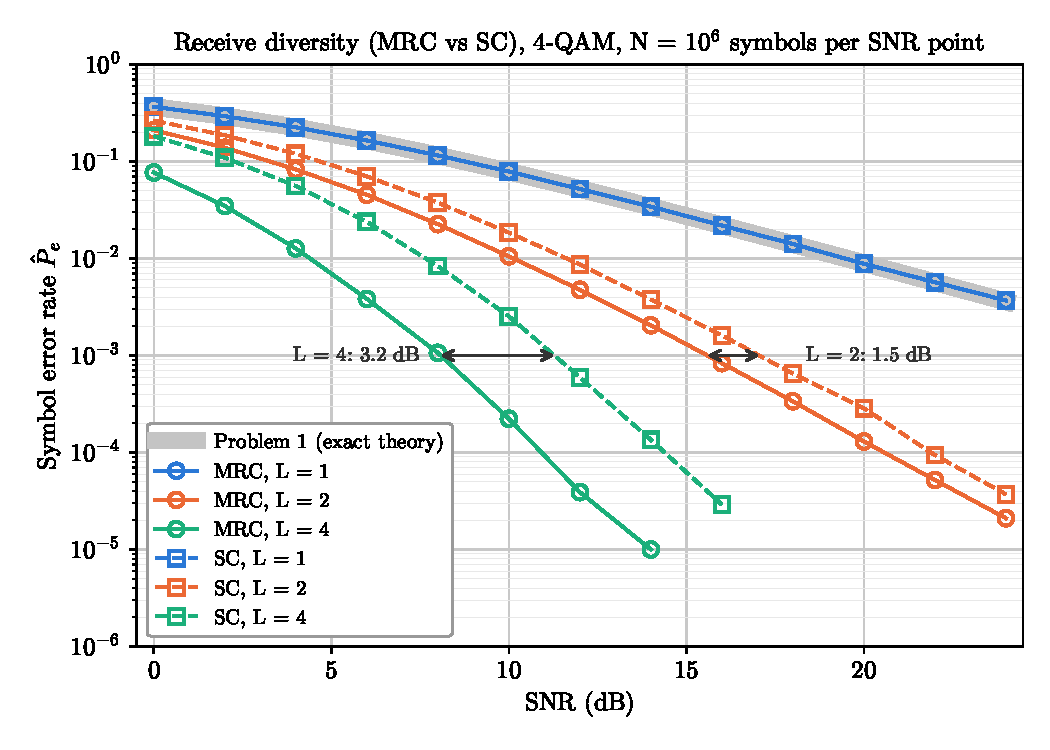
\includegraphics[width=0.74\linewidth]{q2/receive_diversity.pdf}
  \caption{Problem~2: SER of 4-QAM with $L \in \{1, 2, 4\}$ receive antennas. MRC:
           solid lines, circles; SC: dashed lines, squares; one colour per $L$. Grey
           band: exact single-antenna 4-QAM SER of Problem~1. Monte Carlo with
           $N = 10^6$ symbols per SNR point, $\snrdb \in \{0, 2, \dots, 24\}$ (average
           SNR per antenna); points with $\nerr < 10$ are omitted, so the $L = 4$
           curves stop at 14 and 16~dB. Arrows: the MRC--SC gap at $10^{-3}$, 3.2~dB for
           $L = 4$ and 1.5~dB for $L = 2$. \textbf{For each $L$, MRC and SC have the same
           slope, and MRC is better by a nearly constant gap; for $L = 1$ the two curves
           are identical} (Sec.~\ref{sec:p2-gap}).}
  \label{fig:receive}
\end{figure}

\begin{figure}[htbp]
  \centering
  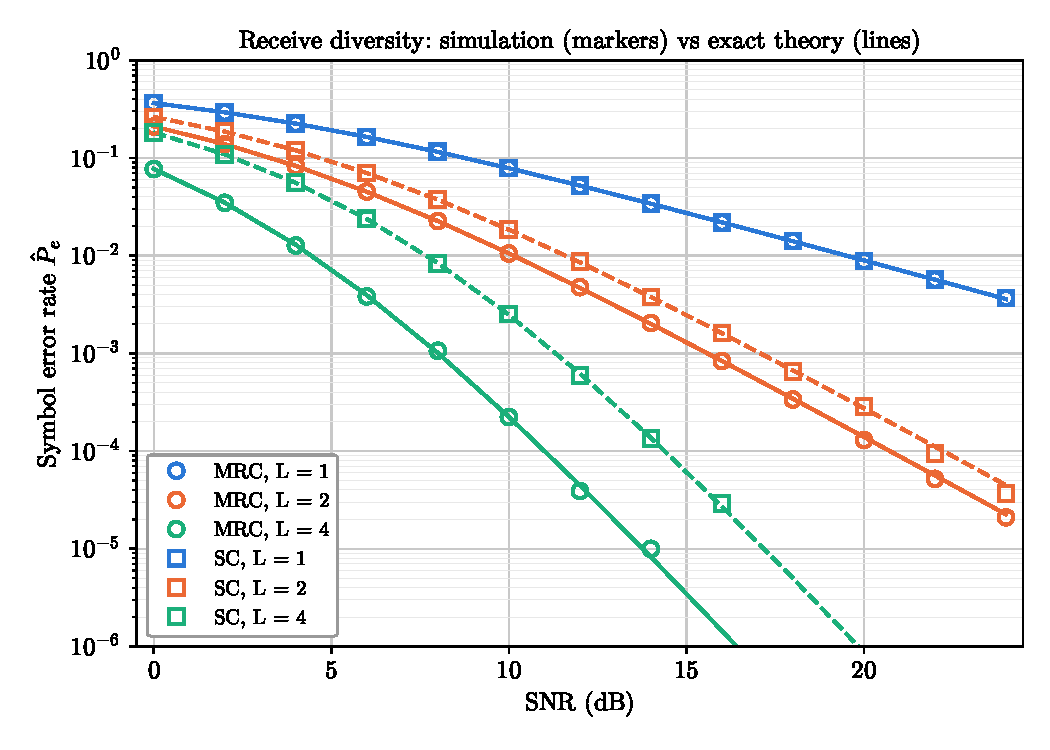
\includegraphics[width=0.74\linewidth]{q2/receive_diversity_theory.pdf}
  \caption{Extra figure: the simulated points of Fig.~\ref{fig:receive} ($N = 10^6$
           symbols per SNR point, 0--24~dB) against the exact theory of
           Sec.~\ref{sec:exact} (lines; MRC solid, SC dashed). \textbf{Every plotted
           point lies on its theory curve} (within $2.01\sigma$).}
  \label{fig:receive-theory}
\end{figure}

\FloatBarrier   % both figures before the discussion
\subsection{Discussion}
\label{sec:p2-discussion}

The assignment asks for four points: the decision statistics of Task~1
(Sec.~\ref{sec:p2-disc-statistics}), a consistency check for $L = 1$
(Sec.~\ref{sec:p2-consistency}), the high-SNR slope of each curve against the
predicted diversity order (Sec.~\ref{sec:p2-slope}), and the SNR gap between MRC and
SC with its origin in array gain (Sec.~\ref{sec:p2-gap}).

\subsubsection{Decision statistics}
\label{sec:p2-disc-statistics}

These are derived in Sec.~\ref{sec:p2-statistics}.
Both receivers give $r = g\,x + n$ with $n \sim \CN(0, 1/\snr)$, so the Problem~1
detector is reused unchanged.

\subsubsection{Consistency check (\texorpdfstring{$L = 1$}{L = 1})}
\label{sec:p2-consistency}
\begin{itemize}
  \item With one antenna, MRC is only a phase rotation, $r = (h^*/\abs{h})\,y$, and SC
        has only one branch to choose. Both reduce to coherent detection on
        $y = hx + w$. They also process the same realisations, so their error counts
        are \emph{identical} at every SNR (checked in the code), and the two curves
        coincide in Fig.~\ref{fig:receive}.
  \item The $L = 1$ curve lies on the 4-QAM fading curve of Problem~1. It agrees
        with the exact theory within $1.85\sigma$, and with an independent re-run of
        the Problem~1 simulation within $1.69\sigma$.
  \item All MRC and SC curves agree with exact theory (Fig.~\ref{fig:receive-theory},
        Table~\ref{tab:a-receive}); every plotted point is within $2.01\sigma$.
\end{itemize}

\subsubsection{High-SNR slope versus diversity order}
\label{sec:p2-slope}

MRC and SC both have diversity
order $L$, i.e.\ $\Pe \propto \snr^{-L}$. An error now needs \emph{all} $L$
independent branches to fade at once. With $\epsilon = 1/\snr$:
\begin{equation}
  \Pr\big[\norm{\h}^2 < \epsilon\big] \approx \frac{\epsilon^L}{L!} \quad\text{(MRC)},
  \qquad
  \Pr\big[\max_\ell \abs{h_\ell}^2 < \epsilon\big] = \big(1 - e^{-\epsilon}\big)^L \approx \epsilon^L \quad\text{(SC)}.
  \label{eq:deep-fade-L}
\end{equation}
Table~\ref{tab:p2-slopes} gives the slope $-\Delta\log_{10}\hPe/\Delta\log_{10}\snr$ at
the high-SNR end of each curve.

\begin{table}[htbp]
  \centering\small
  \caption{High-SNR slopes over the last four points with at least 50 errors:
           local slope of each 2~dB step, least-squares fit through the four
           points, the exact theory fitted over the same points, and the exact theory
           at 60--70~dB.}
  \label{tab:p2-slopes}
  \begin{tabular}{@{}lllcccc@{}}
    \toprule
    & & & \multicolumn{2}{c}{Fitted slope} & Exact theory, & Diversity \\
    \cmidrule(lr){4-5}
    Receiver & Fit range & Local slopes & simulation & exact theory & 60--70~dB & order \\
    \midrule
    MRC / SC, $L = 1$ & 18--24~dB & $1.02,\ 0.95,\ 0.94$ & 0.97 & 0.99 & 1.00 & 1 \\
    MRC, $L = 2$      & 16--22~dB & $1.97,\ 2.07,\ 1.99$ & 2.01 & 1.96 & 2.00 & 2 \\
    SC, $L = 2$       & 16--22~dB & $1.98,\ 1.78,\ 2.42$ & 2.03 & 1.93 & 2.00 & 2 \\
    MRC, $L = 4$      & 4--10~dB  & $2.60,\ 2.78,\ 3.40$ & 2.91 & 2.94 & 4.00 & 4 \\
    SC, $L = 4$       & 8--14~dB  & $2.59,\ 3.15,\ 3.22$ & 3.00 & 2.98 & 4.00 & 4 \\
    \bottomrule
  \end{tabular}
\end{table}

\begin{itemize}
  \item \textbf{$L = 1$ and $L = 2$:} the fitted slopes (0.97, 2.01 and 2.03) are the
        predicted diversity orders 1 and 2. A single 2~dB step is less accurate
        (about $\pm0.2$--$0.3$ with a few hundred errors per point), which explains
        the 1.78 and 2.42 in the SC row.
  \item \textbf{$L = 4$:} the measured slope is about 3, not 4. This is not a
        contradiction: $L$ is the \emph{asymptotic} slope. With $10^6$ symbols the
        $L = 4$ curves can only be measured down to about $10^{-5}$ (up to
        10--14~dB), where they are still bending. Exact theory over the same points
        gives the same slopes (2.94 and 2.98). It reaches 4.00 only at 60--70~dB,
        where $\Pe$ is between $10^{-22}$ and $10^{-28}$, far below anything a
        simulation can reach. The
        slope does grow from 2.6 to 3.4 along the measured part, as expected.
\end{itemize}

\subsubsection{SNR gap between MRC and SC, and array gain}
\label{sec:p2-gap}

The arrows in Fig.~\ref{fig:receive} mark this gap. Table~\ref{tab:p2-gaps} gives the SNR each receiver needs for a target SER.

\begin{table}[htbp]
  \centering\small
  \caption{SNR (dB) needed for a target SER, read off the simulated curves (exact
           theory in brackets), and the gap SC $-$ MRC.}
  \label{tab:p2-gaps}
  \begin{tabular}{@{}llccc@{}}
    \toprule
    & & $\Pe = 10^{-2}$ & $\Pe = 10^{-3}$ & $\Pe = 10^{-4}$ \\
    \midrule
    $L = 2$ & MRC        & 10.13 (10.14) & 15.59 (15.60) & 20.57 (20.73) \\
            & SC         & 11.63 (11.61) & 17.05 (17.09) & 21.89 (22.24) \\
            & \textbf{gap} & \textbf{1.50} (1.47) & \textbf{1.46} (1.49) & \textbf{1.32} (1.50) \\
    \midrule
    $L = 4$ & MRC        & 4.40 (4.46)   & 8.08 (8.01)   & 10.92 (11.02) \\
            & SC         & 7.66 (7.69)   & 11.28 (11.34) & 14.39 (14.40) \\
            & \textbf{gap} & \textbf{3.26} (3.23) & \textbf{3.20} (3.33) & \textbf{3.47} (3.38) \\
    \bottomrule
  \end{tabular}
\end{table}

\begin{itemize}
  \item \textbf{The gap is almost constant for each $L$}: about 1.5~dB for $L = 2$
        and 3.2--3.5~dB for $L = 4$. MRC and SC have the same slope $L$, so their
        curves are parallel at high SNR. (The 1.32~dB at $10^{-4}$ for $L = 2$ is read
        between points with only 52--286 errors, so it is accurate to only about
        $\pm0.2$~dB.)
  \item \textbf{Origin: array gain}, the gain in \emph{average} output
        SNR over one antenna, $\E[\snr_{\mathrm{out}}]/\snr$:
        \begin{itemize}
          \item MRC adds the signals of all $L$ antennas coherently, while the noises
                add incoherently: $\E\norm{\h}^2 = L$, i.e.\ 3.01~dB ($L = 2$) and
                6.02~dB ($L = 4$).
          \item SC throws away the energy received on the other $L - 1$ antennas:
                $\E\max_\ell\abs{h_\ell}^2 = \sum_{k=1}^{L}1/k$, i.e.\ only 1.76~dB
                ($L = 2$) and 3.19~dB ($L = 4$).
          \item The difference, 1.25~dB ($L = 2$) and 2.83~dB ($L = 4$), is most of
                the gap. It also explains why the gap grows with $L$: MRC's array gain
                grows like $L$, SC's only like $\ln L$.
        \end{itemize}
  \item \textbf{Why the gap is a little larger than 1.25 / 2.83~dB.} At high SNR the
        SER depends on how often the output SNR is \emph{small}, not on its mean. By
        \eqref{eq:deep-fade-L}, SC is in a deep fade $L!$ times as often as MRC, so
        its SER is $L!$ times higher. On curves of slope $L$ that is a horizontal
        shift of $10\log_{10}(L!)/L$: 1.51~dB ($L = 2$) and 3.45~dB ($L = 4$). The
        measured gaps lie between the array-gain value and this limit.
  \item \textbf{Between different $L$, the gap is not constant.} The slopes differ (1, 2
        and 4), so the curves for different $L$ spread apart as the SER falls. This
        growing gap is the diversity gain.
\end{itemize}

%% ================================================================ problem 3
\section{Problem 3 --- Transmit diversity (MISO \texorpdfstring{$2 \times 1$}{2 x 1}), 4-QAM}
\label{sec:p3}

Problem~3 moves the two antennas to the transmitter. If antenna $\ell$ sends $s_\ell$
in a channel use, the single receive antenna gets
\begin{equation}
  y = h_1 s_1 + h_2 s_2 + w .
  \label{eq:p3-channel}
\end{equation}
\begin{itemize}
  \item \textbf{Channel:} $h_1, h_2 \sim \CN(0,1)$ i.i.d., known at the receiver, and
        drawn again for every symbol (for every block of two channel uses in Alamouti).
  \item \textbf{Noise:} $w \sim \CN(0, 1/\snr)$.
  \item \textbf{Fair comparison:} every scheme sends a total energy
        $\E\big[\abs{s_1}^2 + \abs{s_2}^2\big] = 1$ per channel use, the same as one
        antenna sending $x$. So $\snr$ is the total transmit energy divided by the noise
        variance.
  \item \textbf{Code:} \code{miso_channel} (\code{common/channel.py}) implements
        \eqref{eq:p3-channel}; the transmitters and receivers are in
        \code{problem3/transmit_diversity.py}. The constellation and the detector of
        Problem~1 are reused.
\end{itemize}
As in Problem~2, every receiver ends with one scalar channel $r = g\,x + n$,
$n \sim \CN(0, 1/\snr)$ \eqref{eq:scalar}. Task~1 derives it for each scheme, Task~2
simulates them, and Sec.~\ref{sec:p3-discussion} discusses the results.

\subsection{Task 1: transmission schemes}
\label{sec:p3-task1}

The table summarises the three schemes, with MRC ($L = 2$) of Problem~2 for
comparison; the derivations follow.

\begin{center}\small
  \begin{tabular}{@{}lcccc@{}}
    \toprule
    Scheme & Channel known at transmitter & Symbol scaling & Gain $g$ & Output SNR \\
    \midrule
    Single antenna  & no  & $s = x$ & $h$ & $\abs{h}^2\snr$ \\
    Beamforming     & yes & $s_\ell = (h_\ell^*/\norm{\h})\,x$ & $\norm{\h}$ & $\norm{\h}^2\snr$ \\
    Alamouti        & no  & $\tfrac{1}{\sqrt2}$ on every entry of $\mathbf{S}$ & $\norm{\h}/\sqrt2$ & $\norm{\h}^2\snr/2$ \\
    MRC, $L = 2$    & --  & $s = x$ (one transmit antenna) & $\norm{\h}$ & $\norm{\h}^2\snr$ \\
    \bottomrule
  \end{tabular}
\end{center}

\subsubsection{Single antenna (reference)}

$s = x$ is sent from one antenna, so $y = hx + w$: the fading channel of Problem~1,
with $g = h$ and output SNR $\abs{h}^2\snr$.

\subsubsection{Transmit beamforming}

\textbf{Weights.} The transmitter knows $(h_1, h_2)$ and sends the same
symbol from both antennas, antenna $\ell$ sending $v_\ell x$ with
\begin{equation}
  \mathbf{v} = \frac{\h^*}{\norm{\h}} = \frac{1}{\sqrt{\abs{h_1}^2 + \abs{h_2}^2}}
  \begin{pmatrix} h_1^* \\ h_2^* \end{pmatrix},
  \qquad
  y = h_1v_1x + h_2v_2x + w = \norm{\h}\,x + w .
  \label{eq:p3-bf}
\end{equation}
\begin{itemize}
  \item Each path arrives with the real, positive gain
        $h_\ell v_\ell = \abs{h_\ell}^2/\norm{\h}$, so the two paths add in phase.
  \item \textbf{Equivalent channel:} $r = y$, gain $g = \norm{\h}$, noise variance
        $1/\snr$, output SNR $\norm{\h}^2\snr$, the same as MRC with $L = 2$. Detection:
        $\hat\imath = \arg\min_i \abs{y - \norm{\h}u_i}^2$.
  \item \textbf{Scaling:} $\norm{\mathbf{v}} = 1$, so the energy per channel use is
        $\abs{v_1x}^2 + \abs{v_2x}^2 = \abs{x}^2$, with mean 1. No further scaling is
        needed.
\end{itemize}

\subsubsection{Alamouti scheme}

\textbf{Transmission matrix.} The transmitter does not know the channel.
Two symbols are sent in two channel uses; rows are channel uses and columns are
antennas:
\begin{equation}
  \mathbf{S} = \frac{1}{\sqrt2}\begin{pmatrix} x_1 & x_2 \\ -x_2^* & x_1^* \end{pmatrix},
  \qquad
  \begin{aligned}
    y_1 &= \tfrac{1}{\sqrt2}\,(h_1x_1 + h_2x_2) + w_1,\\
    y_2 &= \tfrac{1}{\sqrt2}\,(-h_1x_2^* + h_2x_1^*) + w_2 .
  \end{aligned}
  \label{eq:alamouti}
\end{equation}
The channel is constant over the two channel uses of a block and independent
across blocks. Conjugating the second sample gives a linear model whose channel
matrix has orthogonal columns:
\begin{equation*}
  \begin{pmatrix} y_1 \\ y_2^* \end{pmatrix}
  = \frac{1}{\sqrt2}\underbrace{\begin{pmatrix} h_1 & h_2 \\ h_2^* & -h_1^* \end{pmatrix}}_{\mathbf{H}}
    \begin{pmatrix} x_1 \\ x_2 \end{pmatrix}
  + \begin{pmatrix} w_1 \\ w_2^* \end{pmatrix},
  \qquad \mathbf{H}^H\mathbf{H} = \norm{\h}^2\,\mathbf{I}.
\end{equation*}
\textbf{Combining.} The receiver projects onto the two columns (normalised by
$\norm{\h}$):
\begin{equation}
  \begin{aligned}
    r_1 &= \frac{h_1^*y_1 + h_2y_2^*}{\norm{\h}} = \frac{\norm{\h}}{\sqrt2}\,x_1 + n_1,\\
    r_2 &= \frac{h_2^*y_1 - h_1y_2^*}{\norm{\h}} = \frac{\norm{\h}}{\sqrt2}\,x_2 + n_2.
  \end{aligned}
  \label{eq:alamouti-comb}
\end{equation}
\begin{itemize}
  \item The other symbol cancels exactly. The noises
        $n_1 = (h_1^*w_1 + h_2w_2^*)/\norm{\h}$ and
        $n_2 = (h_2^*w_1 - h_1w_2^*)/\norm{\h}$ are independent $\CN(0, 1/\snr)$
        (their covariance is $\mathbf{H}^H\mathbf{H}/(\norm{\h}^2\snr) = \mathbf{I}/\snr$),
        so detecting $x_1$ and $x_2$ separately is ML.
  \item \textbf{Equivalent channel:} each $r_k$ has gain $g = \norm{\h}/\sqrt2$, noise
        variance $1/\snr$ and output SNR $\norm{\h}^2\snr/2$, and is detected by the
        Problem~1 detector.
  \item \textbf{Scaling:} every entry of $\mathbf{S}$ carries $1/\sqrt2$, so a channel
        use carries $(\abs{x_1}^2 + \abs{x_2}^2)/2$, with mean 1, and each antenna
        carries half of it.
  \item The rate is one symbol per channel use, as for a single antenna.
\end{itemize}

\subsubsection{Numerical check of the energy constraint}
\label{sec:p3-energy}

The simulation averages the energy actually sent, $\sum_\ell \abs{s_\ell}^2$, over all
channel uses at every SNR point (\code{results/q3/summary.txt}):
\begin{center}\small
  \begin{tabular}{@{}llcc@{}}
    \toprule
    Scheme & Scaling & Total energy (min / max over SNR points) & Per antenna \\
    \midrule
    Single antenna & $s = x$ & 1.000000 / 1.000000 & 1.0000 \\
    Beamforming    & $s_\ell = (h_\ell^*/\norm{\h})\,x$ & 1.000000 / 1.000000 & 0.5000 / 0.5000 \\
    Alamouti       & entries of $\mathbf{S}$, $\pm x_k^{(*)}/\sqrt2$ & 1.000000 / 1.000000 & 0.5000 / 0.5000 \\
    \bottomrule
  \end{tabular}
\end{center}
All schemes, and MRC (one transmit antenna sending $x$), send exactly the energy of
the single-antenna system. For 4-QAM this holds in every single channel use, not
just on average, because $\abs{x}^2 = 1$ for every point.

\subsection{Task 2: simulation}
\label{sec:p3-task2}

The script \code{problem3/transmit_diversity.py} runs Algorithm~1 for
$\snrdb \in \{0, 2, \dots, 24\}$. For each scheme and SNR:
\begin{enumerate}
  \item draw $N = 10^6$ equiprobable 4-QAM symbols and group them into blocks (one
        symbol per block, or two for Alamouti, giving $N/2 = 5\times10^5$ blocks);
  \item draw one $(h_1, h_2)$ per block and form the antenna signals with the scheme's
        transmitter: \eqref{eq:p3-bf} for beamforming, \eqref{eq:alamouti} for Alamouti;
  \item pass them through \eqref{eq:p3-channel} and record the energy sent;
  \item combine with the scheme's receiver, detect with the Problem~1 detector, and
        count the errors over all $N$ symbols.
\end{enumerate}
The MRC ($L = 2$) curve is simulated with the Problem~2 code. Fig.~\ref{fig:transmit}
shows all four curves on one figure, as the assignment asks; Fig.~\ref{fig:transmit-theory}
compares the same points with the exact theory of Sec.~\ref{sec:exact}. Every curve
agrees with its theory (largest deviation $2.55\sigma$), and beamforming agrees with
the independent MRC simulation within $1.51\sigma$.\footnote{The single-antenna
curve is identical to the $L = 1$ curve of Problem~2. Both scripts start from seed
2026 and draw the symbols, channels and noise in the same order.}

\begin{figure}[htbp]
  \centering
  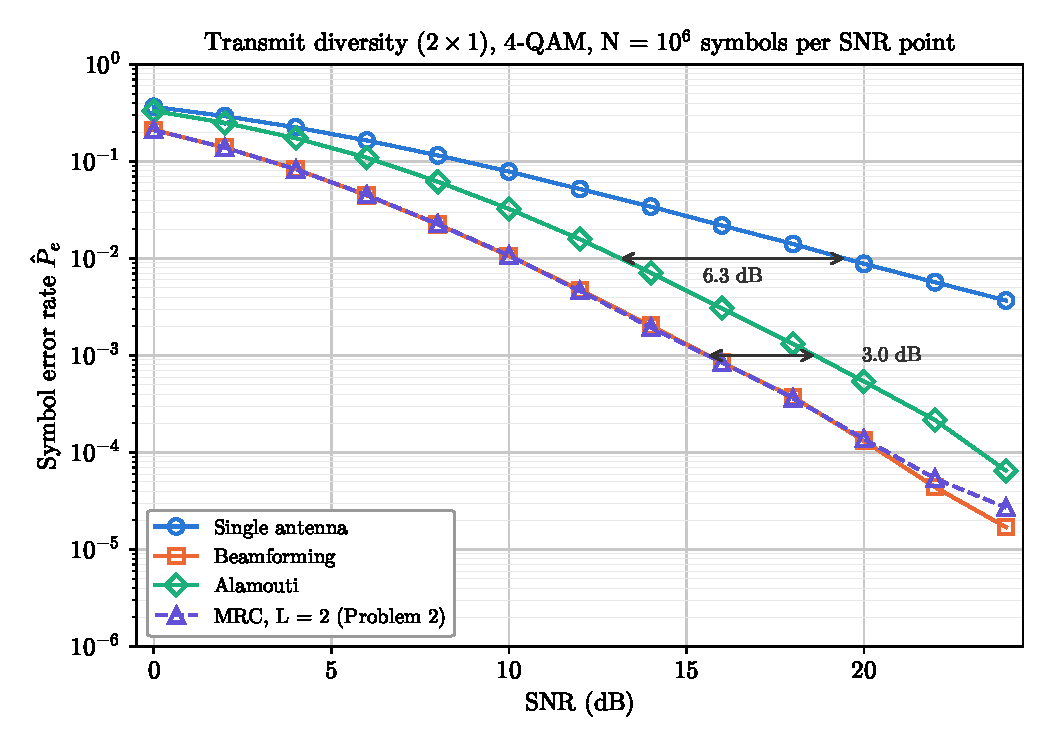
\includegraphics[width=0.74\linewidth]{q3/transmit_diversity.pdf}
  \caption{Problem~3: SER of 4-QAM with a single antenna, transmit beamforming and the
           Alamouti scheme ($2 \times 1$), and MRC with $L = 2$ from Problem~2. All
           schemes transmit a total energy of 1 per channel use. Monte Carlo with
           $N = 10^6$ symbols per SNR point (Alamouti: $5 \times 10^5$ blocks of two
           symbols), $\snrdb \in \{0, 2, \dots, 24\}$; points with $\nerr < 10$ are
           omitted. Arrows: Alamouti is 3.0~dB behind beamforming at $10^{-3}$, and the
           single antenna is 6.3~dB behind Alamouti at $10^{-2}$.
           \textbf{Beamforming and MRC coincide; Alamouti has the same slope but is
           3~dB behind; the gap to the single antenna grows as the SER falls}
           (Sec.~\ref{sec:p3-gaps}).}
  \label{fig:transmit}
\end{figure}

\begin{figure}[htbp]
  \centering
  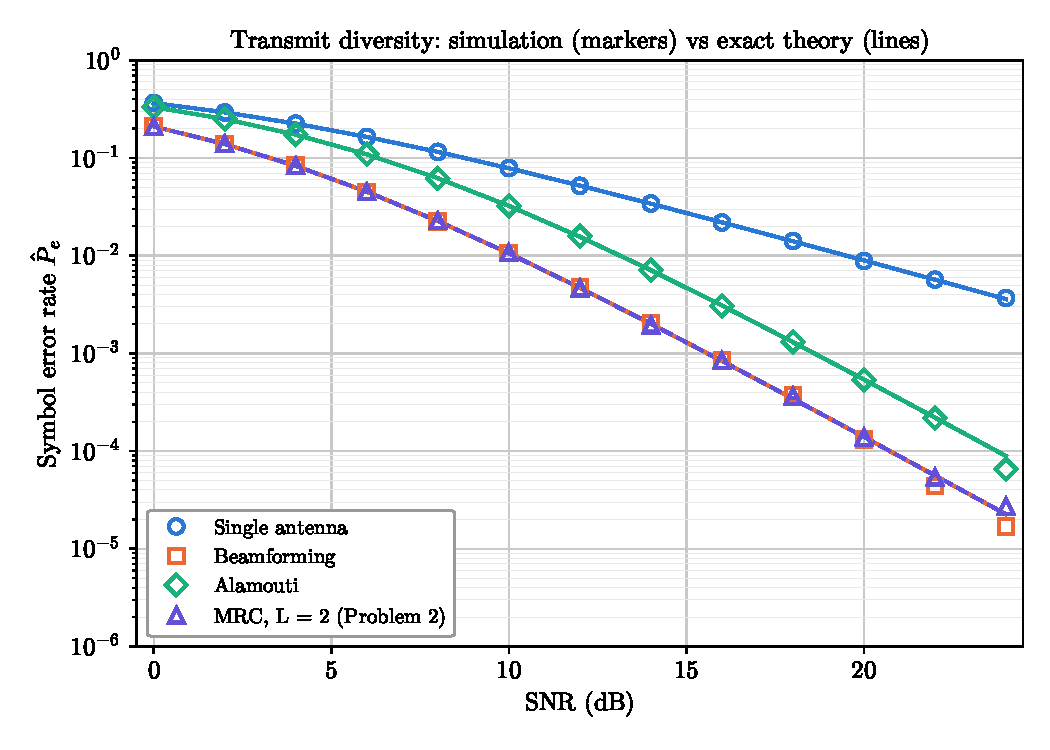
\includegraphics[width=0.74\linewidth]{q3/transmit_diversity_theory.pdf}
  \caption{Extra figure: the simulated points of Fig.~\ref{fig:transmit} ($N = 10^6$
           symbols per SNR point, 0--24~dB) against the exact theory of
           Sec.~\ref{sec:exact} (lines). Beamforming and MRC have the same theoretical
           curve. \textbf{Every plotted point lies on its theory curve} (within
           $2.55\sigma$).}
  \label{fig:transmit-theory}
\end{figure}

\FloatBarrier   % both figures before the discussion
\subsection{Discussion}
\label{sec:p3-discussion}

The assignment asks for two points: the diversity order of each scheme, read from
the slope of its curve at high SNR (Sec.~\ref{sec:p3-diversity}), and the SNR gaps
between beamforming, Alamouti and MRC, with their origin (Sec.~\ref{sec:p3-gaps}).

\subsubsection{Diversity order}
\label{sec:p3-diversity}

Table~\ref{tab:p3-slopes} gives the high-SNR slope of each curve.

\begin{table}[htbp]
  \centering\small
  \caption{High-SNR slopes over the last four points with at least 50 errors, as in
           Table~\ref{tab:p2-slopes}.}
  \label{tab:p3-slopes}
  \begin{tabular}{@{}lllcccc@{}}
    \toprule
    & & & \multicolumn{2}{c}{Fitted slope} & Exact theory, & Diversity \\
    \cmidrule(lr){4-5}
    Scheme & Fit range & Local slopes & simulation & exact theory & 60--70~dB & order \\
    \midrule
    Single antenna & 18--24~dB & $1.02,\ 0.95,\ 0.94$ & 0.97 & 0.99 & 1.00 & 1 \\
    Beamforming    & 14--20~dB & $1.90,\ 1.77,\ 2.26$ & 1.96 & 1.93 & 2.00 & 2 \\
    Alamouti       & 18--24~dB & $1.94,\ 1.99,\ 2.61$ & 2.16 & 1.94 & 2.00 & 2 \\
    MRC, $L = 2$   & 16--22~dB & $1.83,\ 2.10,\ 2.04$ & 2.00 & 1.96 & 2.00 & 2 \\
    \bottomrule
  \end{tabular}
\end{table}

\begin{itemize}
  \item The single antenna has diversity order 1. Beamforming, Alamouti and MRC all
        have diversity order 2.
  \item In all three two-antenna schemes, the output SNR is proportional to
        $\norm{\h}^2 = \abs{h_1}^2 + \abs{h_2}^2$. This is small only if \emph{both}
        paths fade at once, which has probability $\approx \snr^{-2}/2$.
  \item The Alamouti fit (2.16) is pulled up by its last step (2.61), from 216 to only
        65 errors. One 2~dB step with so few errors is accurate to only about
        $\pm0.3$.
  \item Alamouti reaches full diversity even though the transmitter knows nothing
        about the channel.
\end{itemize}

\subsubsection{SNR gaps and their origin}
\label{sec:p3-gaps}

The arrows in Fig.~\ref{fig:transmit} mark two of these gaps.
Table~\ref{tab:p3-gaps} gives the SNR each scheme needs for a target SER.

\begin{table}[htbp]
  \centering\small
  \caption{SNR (dB) needed for a target SER, read off the simulated curves (exact
           theory in brackets), and the gaps between the schemes. ``--'': the curve
           does not reach this SER within 0--24~dB.}
  \label{tab:p3-gaps}
  \begin{tabular}{@{}lccc@{}}
    \toprule
    & $\Pe = 10^{-2}$ & $\Pe = 10^{-3}$ & $\Pe = 10^{-4}$ \\
    \midrule
    Single antenna & 19.46 (19.51) & -- (29.58)    & -- (39.59) \\
    Beamforming    & 10.15 (10.14) & 15.61 (15.60) & 20.51 (20.73) \\
    Alamouti       & 13.15 (13.15) & 18.62 (18.61) & 23.28 (23.75) \\
    MRC, $L = 2$   & 10.17 (10.14) & 15.59 (15.60) & 20.69 (20.73) \\
    \midrule
    Beamforming $-$ MRC      & $-0.02$ (0.00) & $+0.02$ (0.00) & $-0.18$ (0.00) \\
    Alamouti $-$ MRC         & $+2.98$ (3.01) & $+3.03$ (3.01) & $+2.60$ (3.01) \\
    Alamouti $-$ beamforming & $+3.00$ (3.01) & $+3.01$ (3.01) & $+2.78$ (3.01) \\
    Single $-$ Alamouti      & $+6.32$ (6.36) & -- (10.97)     & -- (15.84) \\
    \bottomrule
  \end{tabular}
\end{table}

The $10^{-4}$ column is the least accurate (about $\pm0.3$~dB): there the curves
are interpolated between points with only 44--216 errors.

\begin{itemize}
  \item \textbf{Beamforming = MRC ($L = 2$): constant 0~dB.} Both give the output SNR
        $\norm{\h}^2\snr$.
        \begin{itemize}
          \item With MRC, the receiver collects the signal on two antennas, each with
                its own independent noise.
          \item With beamforming, the transmitter uses its channel knowledge to make
                the two paths add coherently at the single receive antenna.
          \item Both get the same array gain of 2 (3.01~dB, measured 3.01~dB) and
                diversity 2. The measured differences ($\le 0.18$~dB) are Monte Carlo
                noise. The difference lies in what each needs: MRC needs two receive
                chains, beamforming needs channel feedback.
        \end{itemize}
  \item \textbf{Alamouti: a constant 3~dB behind both} (exactly $10\log_{10}2$).
        \begin{itemize}
          \item Without channel knowledge, the transmitter cannot phase-align the two
                antennas. It must split its energy equally ($1/\sqrt2$ per antenna), and
                the two signals do not add coherently.
          \item The output SNR is $\norm{\h}^2\snr/2$, whose mean equals the SNR: array
                gain 1 (0~dB, measured 0.00~dB), but full diversity 2.
          \item This SNR has exactly the beamforming/MRC distribution scaled by
                $1/2$, so
                \begin{equation*}
                  \Pe^{\mathrm{Alamouti}}(\snr) = \Pe^{\mathrm{BF}}(\snr/2).
                \end{equation*}
                The Alamouti curve is the beamforming curve shifted right by 3.01~dB at
                \emph{every} SNR, not only asymptotically. The simulation gives
                3.00 and 3.01~dB at $10^{-2}$ and $10^{-3}$.
          \item These 3~dB are the price of having no channel knowledge at the
                transmitter. In return, Alamouti needs no feedback, still sends one
                symbol per channel use, and is decoded with simple linear processing.
        \end{itemize}
  \item \textbf{Single antenna versus the two-antenna schemes: not constant.} The
        slopes differ (1 against 2), so the gap grows as the SER falls. Relative to
        Alamouti it is 6.3~dB at $10^{-2}$, and (from exact theory) 11.0~dB at
        $10^{-3}$ and 15.8~dB at $10^{-4}$. This is a diversity gain, not an array
        gain: both schemes have array gain 1.
\end{itemize}

%% ================================================================ summary
\section{Summary of the gaps marked in the figures}

Where a gap changes, the two values are those of the two arrows in the figure.

\begin{center}\small
  \setlength{\tabcolsep}{4pt}
  \begin{tabular}{@{}lclcl@{}}
    \toprule
    Curves compared & Fig. & Gap & Constant? & Reason \\
    \midrule
    BPSK vs 4-QAM, AWGN      & \ref{fig:awgn}            & 3.9, 3.3~dB   & No  & tends to 3~dB (half energy per component) \\
    BPSK vs 4-QAM, fading    & \ref{fig:rayleigh}        & 5.6, 5.5~dB   & Yes & parallel slope-1 lines \\
    AWGN vs fading, BPSK     & \ref{fig:awgn-vs-fading}  & 17.3, 25.8~dB & No  & exponential vs $1/\snr$ decay \\
    MRC vs SC, $L = 1$       & \ref{fig:receive}         & 0~dB          & Yes & identical receivers \\
    MRC vs SC, $L = 2$       & \ref{fig:receive}         & 1.5~dB        & Yes & array gain 3.01 vs 1.76~dB \\
    MRC vs SC, $L = 4$       & \ref{fig:receive}         & 3.2~dB        & Yes & array gain 6.02 vs 3.19~dB \\
    Beamforming vs MRC, $L = 2$ & \ref{fig:transmit}    & 0~dB          & Yes & same output SNR \\
    Alamouti vs beamforming  & \ref{fig:transmit}        & 3.0~dB        & Yes & no channel knowledge, so no array gain \\
    Single antenna vs Alamouti & \ref{fig:transmit}      & 6.3~dB        & No  & diversity 1 vs 2: the gap grows \\
    \bottomrule
  \end{tabular}
\end{center}

\textbf{In short:} curves with the same diversity order are parallel at high SNR and
differ by a constant gap (array gain or modulation); curves with different diversity
orders move apart as the SER falls.

%% ================================================================ appendix
\appendix
\section{Numerical results}
\label{app:tables}

The tables are read directly from the CSV files in \code{results/} when the report
is compiled. For Problems~2 and~3 they come from the \code{*_theory.csv} files,
which hold the simulated values and the exact theory side by side.
``sim.'' is $\nerr/N$ with $N = 10^6$. For points with fewer than 10 errors the
raw error count is shown instead (in italics); these points are not plotted.

\begin{table}[htbp]
  \centering\footnotesize
  \caption{Problem~1, AWGN: simulated SER and theory.}
  \label{tab:a-awgn}
  \pgfplotstabletypeset[ser table,
    columns={[index]0,[index]1,[index]5,[index]3,[index]6},
    display columns/1/.style={sim}, display columns/2/.style={theory},
    display columns/3/.style={sim}, display columns/4/.style={theory},
    every head row/.style={
      before row={\toprule & \multicolumn{2}{c}{BPSK} & \multicolumn{2}{c}{4-QAM}\\
                  \cmidrule(lr){2-3}\cmidrule(lr){4-5}},
      after row=\midrule},
  ]{../results/q1/awgn_ser.csv}
\end{table}

\begin{table}[htbp]
  \centering\footnotesize
  \caption{Problem~1, Rayleigh fading: simulated SER and theory. For 4-QAM both the
           table approximation and the exact value are listed.}
  \label{tab:a-rayleigh}
  \pgfplotstabletypeset[ser table,
    columns={[index]0,[index]1,[index]5,[index]3,[index]6,[index]7},
    display columns/1/.style={sim}, display columns/2/.style={theory},
    display columns/3/.style={sim},
    display columns/4/.style={theory, column name={table approx.}},
    display columns/5/.style={theory, column name={exact}},
    every head row/.style={
      before row={\toprule & \multicolumn{2}{c}{BPSK} & \multicolumn{3}{c}{4-QAM}\\
                  \cmidrule(lr){2-3}\cmidrule(lr){4-6}},
      after row=\midrule},
  ]{../results/q1/rayleigh_ser.csv}
\end{table}

\begin{table}[htbp]
  \centering\footnotesize
  \setlength{\tabcolsep}{4pt}
  \caption{Problem~2: simulated 4-QAM SER and exact theory. For $L = 1$, MRC and SC
           give identical results, equal to the single-antenna columns of
           Table~\ref{tab:a-transmit}.}
  \label{tab:a-receive}
  \pgfplotstabletypeset[ser table,
    columns={[index]0,[index]3,[index]14,[index]9,[index]17,[index]5,[index]15,[index]11,[index]18},
    display columns/1/.style={sim}, display columns/2/.style={theory},
    display columns/3/.style={sim}, display columns/4/.style={theory},
    display columns/5/.style={sim}, display columns/6/.style={theory},
    display columns/7/.style={sim}, display columns/8/.style={theory},
    every head row/.style={
      before row={\toprule & \multicolumn{2}{c}{MRC, $L = 2$} & \multicolumn{2}{c}{SC, $L = 2$}
                  & \multicolumn{2}{c}{MRC, $L = 4$} & \multicolumn{2}{c}{SC, $L = 4$}\\
                  \cmidrule(lr){2-3}\cmidrule(lr){4-5}\cmidrule(lr){6-7}\cmidrule(lr){8-9}},
      after row=\midrule},
  ]{../results/q2/receive_diversity_theory.csv}
\end{table}

\begin{table}[htbp]
  \centering\footnotesize
  \setlength{\tabcolsep}{4pt}
  \caption{Problem~3: simulated 4-QAM SER and exact theory.}
  \label{tab:a-transmit}
  \pgfplotstabletypeset[ser table,
    columns={[index]0,[index]1,[index]9,[index]3,[index]10,[index]5,[index]11,[index]7,[index]12},
    display columns/1/.style={sim}, display columns/2/.style={theory},
    display columns/3/.style={sim}, display columns/4/.style={theory},
    display columns/5/.style={sim}, display columns/6/.style={theory},
    display columns/7/.style={sim}, display columns/8/.style={theory},
    every head row/.style={
      before row={\toprule & \multicolumn{2}{c}{Single antenna} & \multicolumn{2}{c}{Beamforming}
                  & \multicolumn{2}{c}{Alamouti} & \multicolumn{2}{c}{MRC, $L = 2$}\\
                  \cmidrule(lr){2-3}\cmidrule(lr){4-5}\cmidrule(lr){6-7}\cmidrule(lr){8-9}},
      after row=\midrule},
  ]{../results/q3/transmit_diversity_theory.csv}
\end{table}

\end{document}
